\chapter{RESULTS}
\label{chapter:results}

\section{The Bean V2 prototype Implementation}
The Bean V2 prototype was designed for a standard mixed-signal $180\text{-nm}$ \textsc{cmos} process. This iteration of the Bean includes two standalone structures: a trimmed version a readout channel, which includes two CSA (one with its input and output connected, to generate the baseline voltage\footnote{The baseline is defined as the CSA DC output voltage after reset, when no input has been applied.}), a pre-charger circuit, the designed SC filter and output buffers; and an isolated version of the filter with its inputs directly bonded out off-chip.  Both structures will be tested separately, thus control signals and reference voltages for both filters are tied together. Also, a logic circuit to generate the non-overlapping two-phase clock was included. Future revisions of the prototype will include a 10-bit SAR ADC and a digital memory within the channel.

Fig.~\ref{fig:IC_layout} shows the layout of the Bean V2 prototype; for a detailed description of the IC pinout, see Appendix~A. Each channel cell was designed to have a pitch lower than $190\,\mu\text{m}$. If the number of channels is increased to the nominal value of $32$, the IC will be approximately $6\,\text{mm}$ tall, which can be fit into four mini@sic sub-blocks according to the Europractice rules. After including the ADC and the digital memory, channel length is expected to be lower than $1\,\text{mm}$.

\begin{figure}[!t]
	\centering
	\includegraphics[width=5in]{./Figures/IC_layout}
	\caption{The Bean V2 prototype layout.}\label{fig:IC_layout}
\end{figure}

The SC filter, shown in Fig.~\ref{fig:filter_layout}, has a total area of $185\,\mu\text{m}\times 332\,\mu\text{m}$, and was laid out to resemble the components spatial distribution of the circuit in Fig.~\ref{fig:filter_post}. The filters outputs, the main CSA output and the baseline voltage are buffered out off-chip using the rail-to-rail amplifiers (connected as unity-gain buffers) shown in Fig.~\ref{fig:buffer_layout}. The CSA and the filter OTA are depicted in Figs.~\ref{fig:csa_layout} and \ref{fig:ota_layout} respectively. All structures were carefully side-shielded with multiple guard-rings. Also, to mitigate the effects of cross-chip gradients,  the \mbox{common-centroid} technique and dummy devices were used in the layout of the filter OTA and the rail-to-rail op-amps. These considerations were not taken into account for the CSA layout, since mismatch is not critical for this cell because of the size of its transistors and because it is a single-ended device. As mentioned in the previous chapter, capacitors $C_F$ and $C_S$ were implemented with a parallel connection of unity MIM capacitors. To prevent copper-dishing effects, both capacitors were surrounded by dummy capacitors implemented with the same unity capacitors.

\begin{figure}[!t]
	\centering
	\includegraphics[width=6in]{./Figures/filter_layout}
	\caption{Filter Layout.}\label{fig:filter_layout}
\end{figure}


\begin{figure}[!p]
	\centering
	\includegraphics[width=4in]{./Figures/CSA_layout}
	\caption{Charge-sensitive amplifier layout. Feedback capacitors are not included here.}\label{fig:csa_layout}
\end{figure}

\begin{figure}[!t]
	\centering
	\includegraphics[width=4.5in]{./Figures/OTA_layout}
	\caption{Recycling folded cascode OTA layout.}\label{fig:ota_layout}
\end{figure}

\begin{figure}[!t]
	\centering
	\includegraphics[width=4.5in]{./Figures/buffer_layout}
	\caption{Rail-to-rail operational amplifier layout.}\label{fig:buffer_layout}
\end{figure}

Because of the lack of models for the pads provided by Faraday and the tools needed to use them, it was necessary to design custom pads. They were designed for ground, positive supply voltage, analog input/output, digital input, and digital output. Special care was taken for the Latch-up failure of the output digital drivers, and the electrostatic discharge phenomena. 

\section{Filter post-layout simulation results}
\subsection{Sub-blocks}
The filter OTA and the buffer op-amp are the complex sub-blocks of the design. Thus, before proceeding with the complete layout, both structures were extracted separately and simulated individually. Figs.~\ref{fig:bode_OTA} and \ref{fig:bode_buffer}  shows the simulated open-loop response of the filter OTA and the buffer op-amp, respectively. The results are very close to the \mbox{pre-layout} simulation results of Chapter \ref{chapter:filter}, the most important difference is that the phase margin of the \mbox{op-amp} is $8^\circ$ lower than the pre-layout estimation. However, it is still within a safe and stable margin. To prove stability, exhaustive transients simulations were run using sharp voltage steps on the inputs, the power supply and the different voltage references. Special care was taken to prove stability of the $\beta$ multiplier circuit.

\begin{figure}[!t]
	\centering
	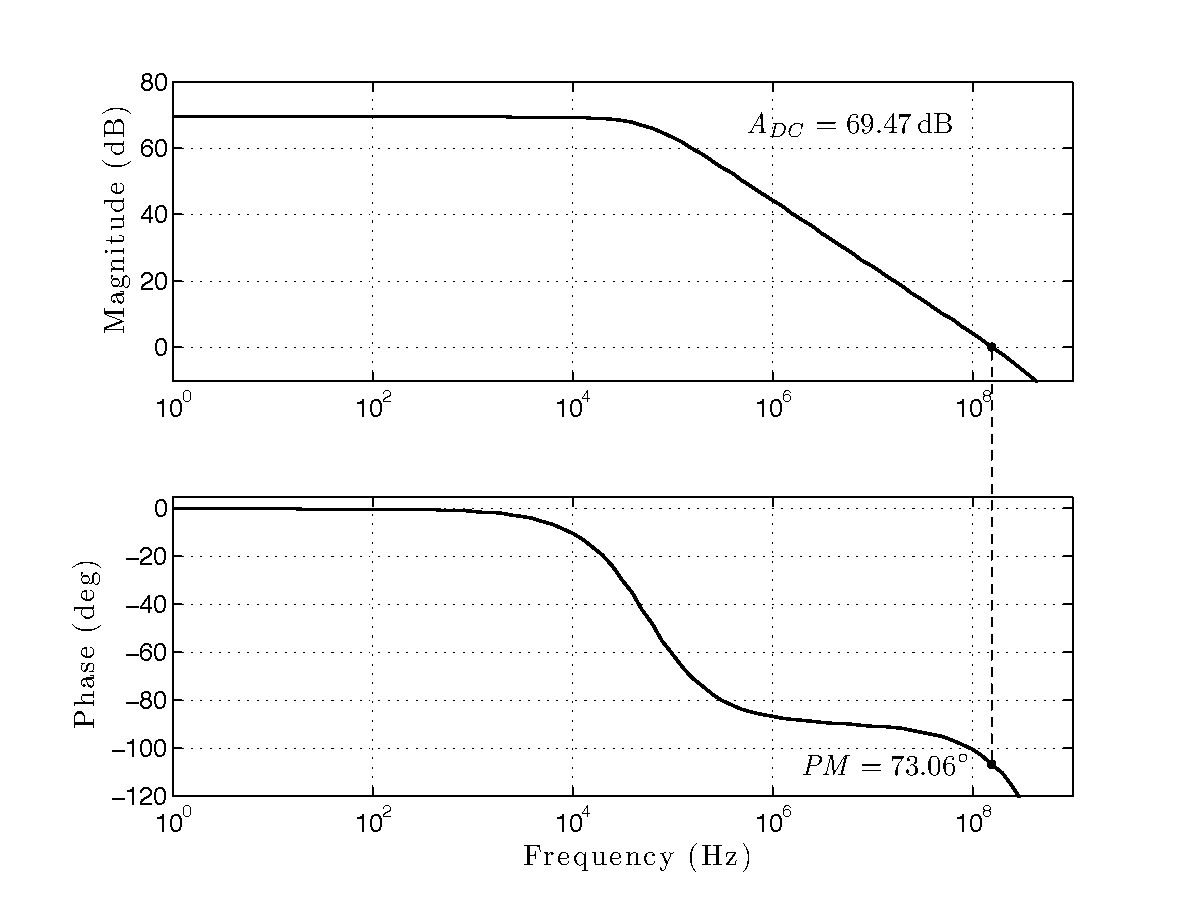
\includegraphics[width=5.3in]{./Test/bode_OTA_post}
	\caption{Bode plot for the OTA open-loop response, with a $0.4\,\text{pF}$ load capacitance.}\label{fig:bode_OTA}
\end{figure}

\begin{figure}[!t]
	\centering
	\includegraphics[width=5.3in]{./Test/bode_buffer_post}
	\caption{Bode plot for the buffer open-loop response, with a $8\,\text{pF}$ load capacitance.}\label{fig:bode_buffer}
\end{figure}

\subsection{Power dissipation} 

The power dissipated by the SC filter prototype was estimated using transient simulations over the extracted filter, under nominal operation and a single input value. The results are presented in Table~\ref{tab:power_dissipation}. The measurements are current consumption averages of the supply node of each component, thus, taking into account dynamic power consumption of the logic circuits.  

\begin{table}
	\begin{center}
		\begin{tabular}{|l|c|}\hline
			{\bf Component} & {\bf Current dissipation} \\ \hline\hline
			%CSA & $2.718\,\text{mW}$ \\ \hline			
			%CSA bias & $0.954\,\text{mW}$ \\ \hline			 
			Filter OTA & $369\,\mu\text{A}$ \\ \hline
			Filter bias and logic & $194\,\mu\text{A}$ \\ \hline
			Unity-gain buffer & $360\,\mu\text{A}$ \\ \hline
		\end{tabular}
		\vspace*{5pt}
		\caption{SC filter simulated current dissipation.}
		\label{tab:power_dissipation}
	\end{center}
\end{table}


\subsection{Functionality} 
A transient simulation using the entire extracted SC filter, including the bias structures, the buffers and the non-overlapping two-phase clock generator, was used to test the filter functionality. Control signals were driven with piecewise-linear voltage sources and a differential voltage step was used as filter input. Fig.~\ref{fig:test_filter_after_omni} shows the simulation result. The measured waveform confirms the functionality of all blocks.

A single clock cycle transient simulation was used to test the variable gain functionality of the filter. The control signals for the variable capacitors were driven with piecewise-linear voltage sources and a differential voltage step was used as filter input. Fig.~\ref{fig:gain_curves} shows the filter step response for the 64 available filter gains. The simulation confirms the monotonically increasing characteristic of the filter gain. However, the increments are not constant between consecutive filter gains. This can be explained due to the use of a binary array to implement the variable capacitor. This could be improved using a thermometer array or a mix between both, at the cost of adding complexity.

\begin{figure}[!t]
	\centering
	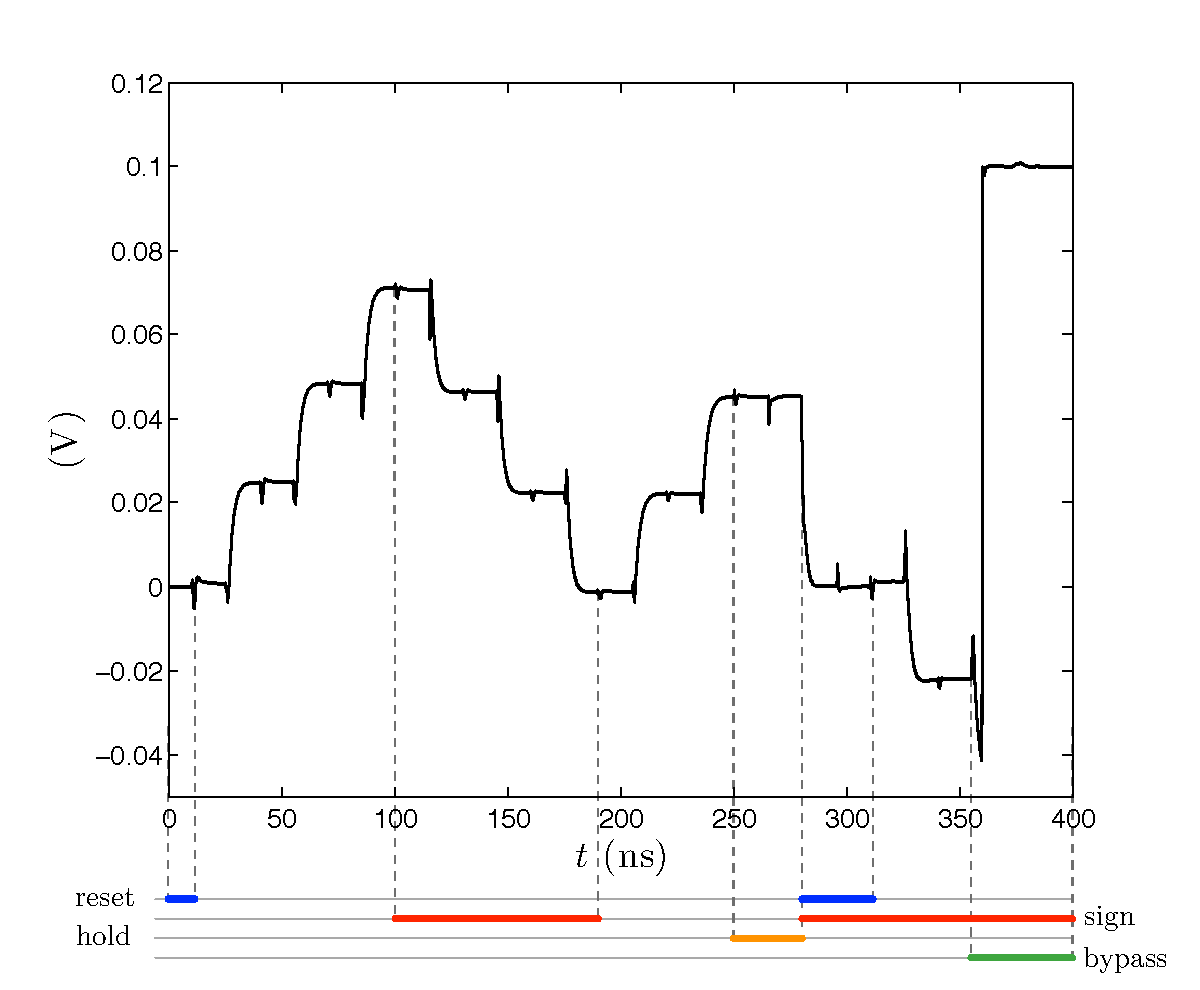
\includegraphics[width=5in]{./Test/test_filter_after_omni.eps}
	\caption{Filter functionality simulation. $V_\textit{in}=0.1\,V$ and $\text{gain}=0.25\,V/V$.}\label{fig:test_filter_after_omni}
\end{figure}

\begin{figure}[!t]
	\centering
	\includegraphics[width=4.4in]{./Test/gain_curves.pdf}
	\caption[Filter step response for constant input for the 64 possible programmable gains.]{Filter step response for constant input for the 64 possible programmable gains. \mbox{$V_\textit{in}=0.1\,V$} and \mbox{$T_s=40\,\text{ns}$}.}\label{fig:gain_curves}
\end{figure}

\subsection{Linearity}
The filter Integral nonlinearity (INL) was simulated for an input ramp covering $100\%$ of the filter input range. The simulations were carried out for nominal speed, with an input ramp driven by an ideal voltage source. Fig.~\ref{fig:inl} shows the simulation result. The INL plot shows a typical second order non-linear behavior caused by variations over the filter OTA gain due to the input range. This can be improved with a constant-$g_m$ OTA input stage and by increasing the OTA open-loop gain.  Spikes on the INL plot are caused by simulation numerical errors, thus they do not represent any filter dysfunction. The high value of the INL is due to the insufficient time for the filter to settle. Future revision of the Bean should consider the filter dynamical behavior and take special attention to the common-mode feedback loop, which was one of the factors that affected the filter settling time in this iteration of the design. 

\begin{figure}[!t]
	\centering
	\includegraphics[width=4.4in]{./Test/linearity.pdf}
	\caption{Filter linearity simulation results, full-scale input range.}\label{fig:inl}
\end{figure}

\subsection{Weighting function}
The filter weighting function (WF) was simulated according to its definition described in Chapter~\ref{chapter:theoretical}. This was done by applying an input voltage step at different times within a cycle, and measuring the output at the measurement time. A simple $RC$ network was used to simulate a voltage step as seen at the output of a CSA. Fig.~\ref{fig:wf_test_circuit} shows the circuit used to perform this measurement. 

Fig.~\ref{fig:sim_wf} shows the post-layout SPICE-simulated WF of the filter using flat coefficients and the Bean nominal clock frequency. As expected, its shape resembles the shape of the WFs in Fig.~\ref{fig:optimum_wf},  which confirm the functionality of the filter to synthesize practical WFs. The initial non-zero value is caused by the successive integration of the filter input-referred offset voltage and the filter nonlinearities. Future revision of the filter could include a chopper-stabilized OTA to reduce the offset, and thus, to reduce the WF nonideality.

\begin{figure}[!t]
	\centering
	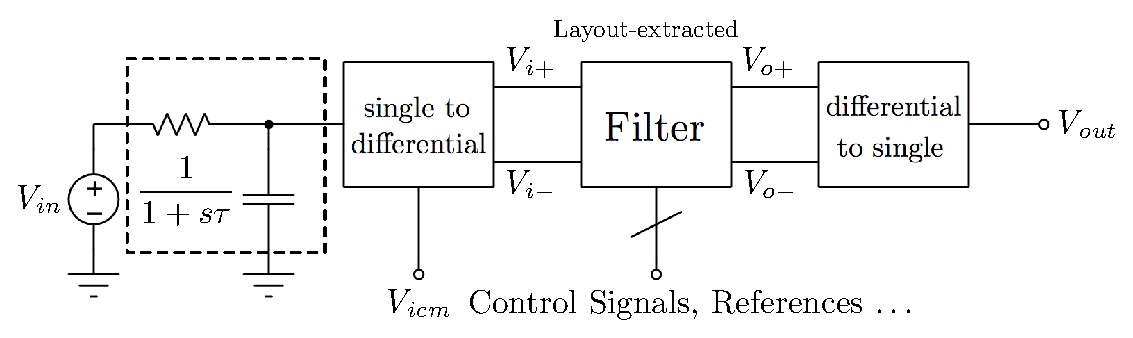
\includegraphics[width=5in]{./Test/wf_test_circuit}
	\caption{Weighting function test circuit.}\label{fig:wf_test_circuit}
\end{figure}

\begin{figure}[!t]
	\centering
	\includegraphics[width=3.6in]{./Test/sim_wf}
	\caption{SPICE-simulated weighting function. $\tau=8\,\text{ns}$, $N=16$ and $T_s=19.25\,\text{ns}$.}\label{fig:sim_wf}
\end{figure}








